\section{Kalman Filters}
\begin{figure}[!htb]
\centering
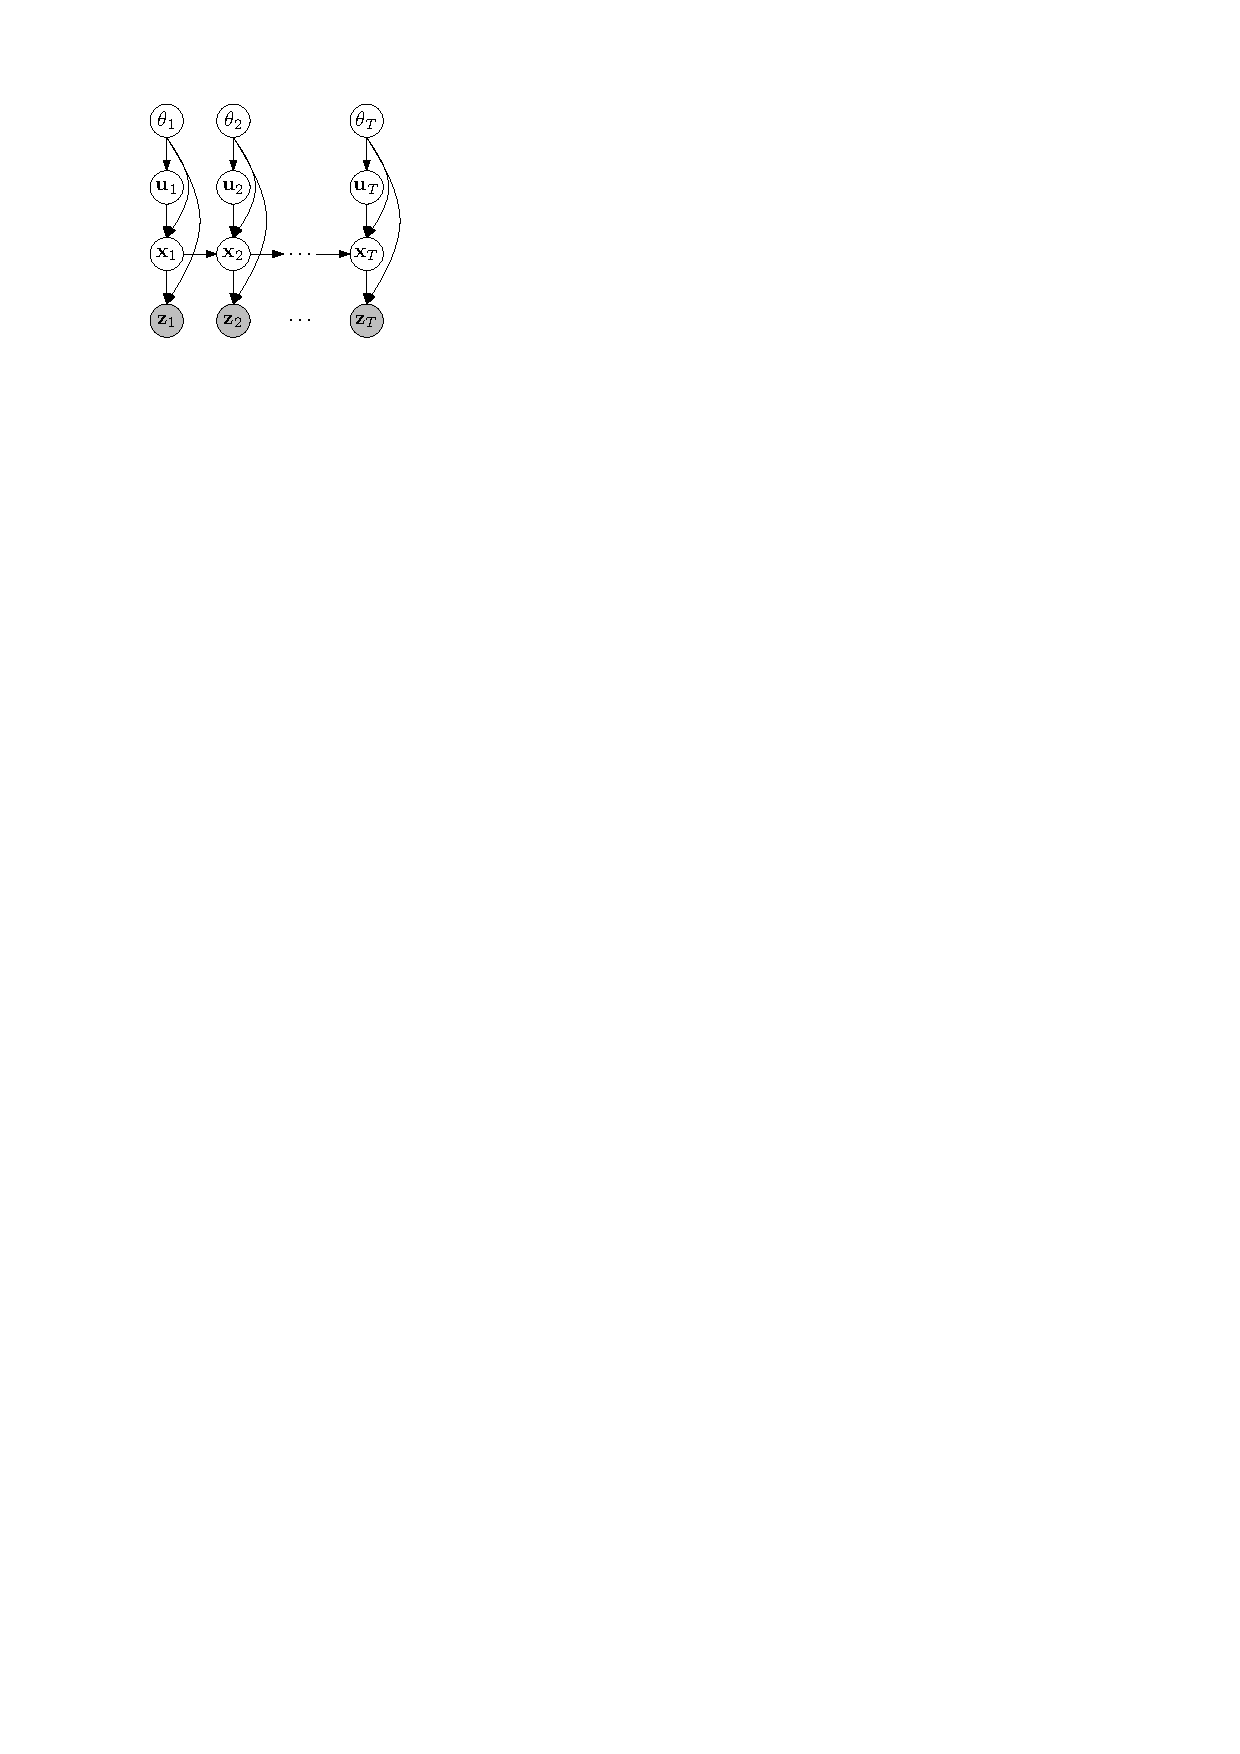
\includegraphics[scale=1]{models/kf/figures/kf}
\caption{Probabilistic Graphical Model for the Kalman Filter.}
\label{fig:models/kf/figures/kf}
\end{figure}

\subsection{Linear Kalman Filter}
The model is, for $t = 1, \dotsc, T$:
\begin{align}
	\vec x_t 		&= \vec A_t \vec x_{t - 1} + \vec B_t \vec u_t + \vec\epsilon_t, & \vec x_t \in \mathbb R^n\\
	\vec z_t		&= \vec C_t \vec x_t + \vec D_t \vec u_t + \vec\delta_t, & \vec z_t \in \mathbb R^m\\
	\vec\epsilon_t	&\sim \Gauss(\vec 0, \vec Q_t) \\
	\vec\delta_t	&\sim \Gauss(\vec 0, \vec R_t) \\
	\vec\theta_t 	&= \{\vec A_t, \vec B_t, \vec C_t, \vec D_t, \vec Q_t, \vec R_t\}
\end{align}

The posteriors of interest are (we drop the conditional dependence on $\vec \theta_t$'s):
\begin{align}
	p(\vec x_t \mid \vec z_{1:t - 1}, \vec u_{1:t})	&= \Gauss\left(\vec x_t \mid \vec \mu_{t \mid t - 1}, \vec\Sigma_{t \mid t - 1}\right) \\
	\vec \mu_{t \mid t - 1}							&= \vec A_t \vec\mu_{t - 1 \mid t - 1} + \vec B_t \vec u_t \\
	\vec \Sigma_{t \mid t - 1}						&= \vec A_t \vec\Sigma_{t - 1 \mid t - 1} \vec A_t^T + \vec Q_t \\
	p(\vec x_t \mid \vec z_{1:t}, \vec u_{1:t}) 	&= \Gauss\left(\vec x_t \mid \vec \mu_{t \mid t}, \vec\Sigma_{t \mid t}\right) \\
	\vec \mu_{t \mid t}								&= \vec\mu_{t \mid t - 1} + \vec K_t \vec r_t \\
	\vec \Sigma_{t \mid t}							&= (\vec I - \vec K_t \vec C_t) \vec\Sigma_{t \mid t - 1} \\
	\vec r_t 										&= \vec z_t - (\vec C_t \vec \mu_{t \mid t - 1} + \vec D_t \vec u_t) \\
	\vec K_t										&= \vec\Sigma_{t \mid t - 1} \vec C_t^T \vec S_t^{-1} \\
	\vec S_t										&= \vec C_t \vec\Sigma_{t \mid t - 1}\vec C_t^T + \vec R_t
\end{align}

\subsubsection{Derivations}

\subsection{Extended Kalman Filter}
The model is , for $t = 1, \dotsc, T$:
\begin{align}
	\vec x_t	&= \vec g(\vec x_{t - 1}, \vec u_t) + \vec \epsilon_t \\
	\vec z_t	&= \vec h(\vec x_t, \vec u_t) + \vec \delta_t \\
	\vec\epsilon_t	&\sim \Gauss(\vec 0, \vec Q_t) \\
	\vec\delta_t	&\sim \Gauss(\vec 0, \vec R_t)
\end{align}

The posteriors of interest are (we drop the conditional dependence on $\vec \theta_t$'s):
\begin{align}
	p(\vec x_t \mid \vec z_{1:t - 1}, \vec u_{1:t})	&\approx \Gauss\left(\vec x_t \mid \vec \mu_{t \mid t - 1}, \vec\Sigma_{t \mid t - 1}\right) \\
	\vec \mu_{t \mid t - 1}							&\approx \vec g(\vec \mu_{t - 1 \mid t - 1}, \vec u_t) \\
	\vec \Sigma_{t \mid t - 1}						&\approx \vec G_t \vec \Sigma_{t - 1 \mid t - 1} \vec G_t^T + \vec Q_t \\
	p(\vec x_t \mid \vec z_{1:t}, \vec u_{1:t}) 	&\approx\ \Gauss\left(\vec x_t \mid \vec \mu_{t \mid t}, \vec\Sigma_{t \mid t}\right) \\
	\vec \mu_{t \mid t}								&\approx \vec \mu_{t \mid t - 1} + \vec W \left(\vec z_t - \vec h(\vec \mu_{t \mid t - 1}, \vec u_t)\right) \\
	\vec \Sigma_{t \mid t}							&\approx \vec \Sigma_{t \mid t - 1} - \vec W \vec S \vec W^T
\end{align}

Note that we make two types of approximations: (1) we assume the posteriors are Gaussians (which they are not) and (2) we calculate the moments using linearised versions of random variables of interest. We define previously undefined variables below.

\subsubsection{Derivations}
The derivation of the prediction equations is as follows:
\begin{align}
	\vec \mu_{t \mid t - 1}	&= \E\left[\vec x_t \mid \vec z_{1:t - 1}, \vec u_{1:t}\right] \\
							&= \E\left[\vec g(\vec x_{t - 1}, \vec u_t) + \vec \epsilon_t \mid \vec z_{1:t - 1}, \vec u_{1:t}\right] \\
							&= \E\left[\vec g(\vec \mu_{t - 1 \mid t - 1}, \vec u_t) + \vec G_t (\vec x_{t - 1} - \vec \mu_{t - 1 \mid t - 1}) + \cdots + \vec \epsilon_t \mid \vec z_{1:t - 1}, \vec u_{1:t}\right]
\end{align}
We have linearised around $\vec \mu_{t - 1 \mid t - 1}$ where $\vec G_t$ is the Jacobian of $\vec g(\vec x, \vec u)$ w.r.t. $\vec x$ evaluated at $\vec \mu_{t - 1 \mid t - 1}$:
\begin{align}
	\vec G_t	&\triangleq \frac{\partial \vec g(\vec x, \vec u)}{\partial \vec x}\at[\bigg]{\vec x = \vec \mu_{t - 1 \mid t - 1}, \vec u = \vec u_t}
\end{align}
i.e. $\frac{\partial \vec g(\vec x, \vec u)}{\partial \vec x} \in \mathbb R^{n \times n}$ and the $(i, j)^{\text{th}}$ element is $\frac{\partial g_i(\vec x, \vec u)}{\partial x_j}$. Taking only the first two terms of the Taylor expansion and continuing with the derivation:
\begin{align}
	\vec \mu_{t \mid t - 1}	&\approx \E\left[\vec g(\vec \mu_{t - 1 \mid t - 1}, \vec u_t) + \vec G_t (\vec x_{t - 1} - \vec \mu_{t - 1 \mid t - 1}) + \vec \epsilon_t \mid \vec z_{1:t - 1}, \vec u_{1:t}\right] \\
							&\,\,\,\vdots \\
							&= \vec g(\vec \mu_{t - 1 \mid t - 1}, \vec u_t)
\end{align}
Similarly, the prediction equation for the covariance can be derived as follows:
\begin{align}
	\vec \Sigma_{t \mid t - 1}	&= \var\left[\vec x_t \mid \vec z_{1:t - 1}, \vec u_{1:t}\right] \\
								&= \var\left[\vec g(\vec x_{t - 1}, \vec u_t) + \vec \epsilon_t \mid \vec z_{1:t - 1}, \vec u_{1:t}\right] \\
								&= \var\left[\vec g(\vec \mu_{t - 1 \mid t - 1}, \vec u_t) + \vec G_t (\vec x_{t - 1} - \vec \mu_{t - 1 \mid t - 1}) + \cdots + \vec \epsilon_t \mid \vec z_{1:t - 1}, \vec u_{1:t}\right] \\
								&\approx \var\left[\vec g(\vec \mu_{t - 1 \mid t - 1}, \vec u_t) + \vec G_t (\vec x_{t - 1} - \vec \mu_{t - 1 \mid t - 1}) + \vec \epsilon_t \mid \vec z_{1:t - 1}, \vec u_{1:t}\right] \\
								&\,\,\,\vdots \\
								&= \vec G_t \vec \Sigma_{t - 1 \mid t - 1} \vec G_t^T + \vec Q_t
\end{align}

The derivation of the update equations is as follows:
\begin{align}
	\vec \mu_{t \mid t}	&= \E\left[\vec x_t \mid \vec z_{1:t}, \vec u_{1:t}\right] \\
						&= \E\left[\vec g(\vec x_{t - 1}, \vec u_t) + \vec \epsilon_t \mid \vec z_{1:t}, \vec u_{1:t}\right] \\
						&= \E\left[\vec g(\vec \mu_{t \mid t - 1}, \vec u_t) + \vec G_t (\vec x_{t - 1} - \vec \mu_{t \mid t - 1}) + \cdots + \vec \epsilon_t \mid \vec z_{1:t}, \vec u_{1:t}\right] \\
						&\approx \E\left[\vec g(\vec \mu_{t \mid t - 1}, \vec u_t) + \vec G_t (\vec x_{t - 1} - \vec \mu_{t \mid t - 1}) + \vec \epsilon_t \mid \vec z_{1:t}, \vec u_{1:t}\right] \\
						&\,\,\,\vdots \\
						&= \vec \mu_{t \mid t - 1} + \vec W \left(\vec z_t - \vec h(\vec \mu_{t \mid t - 1}, \vec u_t)\right) \\
	\vec \Sigma_{t \mid t}	&= \var\left[\vec x_t \mid \vec z_{1:t}, \vec u_{1:t}\right] \\
							&= \var\left[\vec g(\vec x_{t - 1}, \vec u_t) + \vec \epsilon_t \mid \vec z_{1:t}, \vec u_{1:t}\right] \\
							&= \var\left[\vec g(\vec \mu_{t \mid t - 1}, \vec u_t) + \vec G_t (\vec x_{t - 1} - \vec \mu_{t \mid t - 1}) + \cdots + \vec \epsilon_t \mid \vec z_{1:t}, \vec u_{1:t}\right] \\
							&\approx \var\left[\vec g(\vec \mu_{t \mid t - 1}, \vec u_t) + \vec G_t (\vec x_{t - 1} - \vec \mu_{t \mid t - 1}) + \vec \epsilon_t \mid \vec z_{1:t}, \vec u_{1:t}\right] \\
							&\,\,\,\vdots \\
							&= \vec \Sigma_{t \mid t - 1} - \vec W \vec S \vec W^T
\end{align}